%***********************************************************************
% Lab Report Template
% R. W. Melton
% May 19, 2019
% August 24, 2020
%***********************************************************************
%Modify the following macros to set document property values
%used for cover sheet (title page) and page header
\newcommand{\CourseNumber}{CMPE-250}
\newcommand{\CourseName}{Assembly and Embedded Programming}
\newcommand{\SemesterName}{Fall 2020}
\newcommand{\SemesterCode}{20201}
\newcommand{\LabExNum}{10}
\newcommand{\LabExTitle}{Timer driver}
\newcommand{\StudentName}{Andrei Tumbar}
\newcommand{\DateSubmit}{Submitted: 11-10-20}
\newcommand{\LabSection}{5}
\newcommand{\LabInstructor}{Gordon Werner}
\newcommand{\TAa}{Tianran Cui}
\newcommand{\TAb}{Anthony Bacchetta}
\newcommand{\LectureSection}{1}
\newcommand{\LectureInstructor}{Melton}
%End macros for document property values
%***********************************************************************
\title{Lab Ex. \LabExNum\ Report}
\author{\StudentName}
\date{\DateSubmit}
\makeatletter %make \title, \author, and \date availabile with \@
\newcommand{\FontSize}{12}
\newcommand{\FontUnit}{pt}
\newcommand{\HeadSize}{\dimexpr \FontSize\FontUnit + 2pt \relax}
\documentclass[\FontSize\FontUnit,letterpaper,oneside]{article}
\usepackage[twoside=false,margin=1in]{geometry}
\usepackage[utf8]{inputenc}
\usepackage[USenglish]{babel}
\usepackage{graphicx}
\usepackage[normalem]{ulem}
\usepackage{newtxtext, newtxmath}
%If newtx package had to be installed in multiuser environment
%regular user may have to run updmap command to avoid following error
%FATAL:  ``PK font ts1-qtmr could not be created.'' in miktex-makepk
%Alternatively, uncomment the following line
%\pdfmapfile{=pdftex35.map
\usepackage{booktabs}
\usepackage{enumitem}
\usepackage{nameref}
\usepackage{hhline}
\usepackage{fontspec,kantlipsum}
\usepackage[T1]{fontenc}
\usepackage{caption}
\captionsetup[table]{skip=10pt}
\usepackage[pdfborder={0 0 0},plainpages=false,pdfpagelabels]{hyperref}
\def\code#1{\texttt{#1}}
%If hyperref generates errors on first build, rebuild.            
\hypersetup{pdfauthor={\@author},
            pdftitle={\@title},
            pdfsubject={\CourseNumber\ \SemesterCode},
            %pdfkeywords={},
            %pdfproducer={Latex with hyperref, or other system},
            %pdfcreator={pdflatex, or other tool}
            urlcolor=none}
\setlength{\topsep}{\z@}
\setlength{\partopsep}{\z@}
\setlength{\itemsep}{\z@}
\setlength{\parindent}{\z@}
\setlength{\parskip}{\FontSize\FontUnit plus 2pt minus 1pt}
\setlength{\baselineskip}{\dimexpr \FontSize\FontUnit + 2pt \relax}
\renewcommand \baselinestretch{1}
\makeatletter
  \renewcommand \section{
    \@startsection{section}{1}{\z@}
      %Before 2 lines, accounting for normal \parskip
      {\dimexpr \FontSize\FontUnit * 2 - \parskip \relax plus 0pt minus 0pt}
      %After 1 line, accounting for normal \parskip
      {0.1pt plus 2pt minus 1pt} %nonzero amount to get normal \parskip
      {\normalfont\normalsize\bfseries}} 
  \renewcommand \subsection{
    \@startsection{paragraph}{2}{\z@}
      %Before 1 lines, accounting for normal \parskip
      {0.1pt plus 2pt minus 1pt}
      %After 0.5 em on same line as heading
      {-0.5em} 
      {\normalfont\normalsize\bfseries}} 
  \renewcommand \subsubsection{
    \@startsection{paragraph}{3}{\z@}
      %Before 1 line, accounting for normal \parskip
      {0.1pt plus 2pt minus 1pt}
      %After 0.5 em on same line as heading
      {-0.5em} 
      {\normalfont\normalsize\uline}} 
  \renewcommand \paragraph{
      \@startsection{paragraph}{4}{\z@}
      %Before 1 line, accounting for normal \parskip
      {0.1pt plus 2pt minus 1pt}
      %After 0.5 em on same line as heading
      {-0.5em} 
      {\normalfont\normalsize}} 
\makeatother
\pagenumbering{arabic}
\headheight=\HeadSize
\usepackage{fancyhdr}
\renewcommand{\headrulewidth}{0pt}
\renewcommand{\footrulewidth}{0pt}
\makeatletter %make \title, \author, and \date availabile with \@
\pagestyle{fancy}
\fancyhead{} %clear all header fields
\fancyhead[L]{\small \CourseNumber\ \SemesterCode \@author:  \@title}
\fancyhead[R]{\small Page \thepage\ of \pageref*{LastPage}}
\fancyfoot{} %clear all footer fields
\fancypagestyle{plain}{
  \renewcommand{\headrulewidth}{0pt}
  \renewcommand{\footrulewidth}{0pt}
  \fancyhf{} %clear header and footer fields
  \fancyfoot[C]{\small \CourseNumber\ \SemesterCode\ \@author:  \@title:  
    Page \thepage\ of \pageref*{LastPage}}
}
%May require second build to get correct page numbers.   


\usepackage{xcolor}
\usepackage{listings}

\definecolor{mGreen}{rgb}{0,0.6,0}
\definecolor{mGray}{rgb}{0.5,0.5,0.5}
\definecolor{mPurple}{rgb}{0.58,0,0.82}
\definecolor{backgroundColour}{rgb}{0.95,0.95,0.92}

\lstdefinestyle{CStyle}{
    commentstyle=\color{mGreen},
    keywordstyle=\color{magenta},
    numberstyle=\tiny\color{mGray},
    stringstyle=\color{mPurple},
    basicstyle=\footnotesize,
    breakatwhitespace=false,         
    breaklines=true,                 
    captionpos=b,                    
    keepspaces=true,                 
    numbers=left,                    
    numbersep=5pt,                  
    showspaces=false,                
    showstringspaces=false,
    showtabs=false,                  
    tabsize=2,
    language=C
}

         
\begin{document}
\raggedbottom
\widowpenalties 1 10000
\lefthyphenmin=4
\righthyphenmin=4
\setlist{nolistsep}
%***********************************************************************
%Title page is automatically generated from macros at top of file
\pagenumbering{roman}
\begin{titlepage}
  %No space before paragraph at top of page
  %\vspace{\dimexpr-2\parsep-2\parskip\relax}
  %1.5 in before center (list) at top of page
  \vspace*{\dimexpr 1.5in - \topsep - \partopsep - \topskip - \parskip \relax}
  \begin{center}
    \textbf{\large\CourseNumber\ \CourseName\linebreak
      \linebreak
      Laboratory Exercise \LabExNum\linebreak
      \linebreak
      \LabExTitle}
  \end{center}
  \vspace*{\dimexpr 1.5in - \topsep - \partopsep - \topskip \relax}
  \par By submitting this report, I attest that its contents are wholly 
    my individual writing about this exercise and that they reflect 
    the submitted code.  I further acknowledge that permitted 
    collaboration for this exercise consists only of discussions of 
    concepts with course staff and fellow students.  Other than code 
    provided by the instructor for this exercise, all code was 
    developed by me.
  \null
  \vspace*{4\parskip}
  \hspace*{3.25in}\begin{tabular}[t]
    {@{\hskip0pt}r    %Specification
     @{\hskip1em}l    %Value
     @{\hskip0pt}}
    \toprule[1pt]
    \multicolumn{2}{l}{\StudentName}\\
    \multicolumn{2}{l}{\DateSubmit}\\
    \\
    Lab Section:&\LabSection\\
    Instructor:&\LabInstructor\\
    TA:&\TAa\\
    &\TAb\\
    \\
    Lecture Section:&\LectureSection\\
    Lecture Instructor:&\LectureInstructor
  \end{tabular}
\end{titlepage}
\pagenumbering{arabic}
\thispagestyle{plain}
%***********************************************************************
%Report body begins here
\section*{Abstract}
In this laboratory exercise, a timer driver was implemented. The driver utilized the an interrupt driver timing design where a hardware driven peripheral device would interrupt the running program. The interrupt would increment a counter if the timing functionality was enabled. This exercise was successful as the goal to produce a timer accurate to the nearest 10ms was achieved. 


\section*{Procedure}
A command prompt was written that accepted commands: \code{T}, \code{P}, \code{D}, and \code{C} respresented timer start, pause, display, and clear respectively. The timer start command would enable a counter to increment every time the timing interrupt was run. This interrupt was setup to fire every 10ms.
The pause command would stop the timing interrupt from incrementing the counter. The pause however, does not stop the interrupt from firing.
The display command simply displayed the value of the counter in decimal representation.
Finally the clear command cleared the counter to zero.

The counter was initialized to zero at the start of the program. We are using a 32-bit counter to allow the timer to time a long duration.

\section*{Results}
Memory ranges for various parts of the code were found.

\begin{table}[h!]
\begin{center}
\caption{Code section offsets and endings.}
\label{tab:q1}
\begin{tabular}{ |l||c|c| }
\hline
Subroutine & Address & Ending Address \\\hhline{|=||=|=|}
Executable Code & \code{0x00000410} & \code{0x00000923} \\\hline 
PIT ISR & \code{0x00000753} & \code{0x00000768} \\\hline 
Constants in ROM & \code{0x000001c4} & \code{0x0000029b} \\\hline
RAM & \code{0x1ffffd00} & \code{0x1ffffd6f} \\\hline
\end{tabular}
\end{center}
\end{table}

As seen in Table \ref{tab:q1}, the total size of the executable code was around 1.3k. The \code{PIT\_ISR} was just 22 bytes as it was very simple subroutine. The constants contained some of the test prompts used in other labs making the total size 216 bytes. Finally the RAM section was reduced to a size of 112 bytes by decreasing the size of the print queues. The \code{RxQueue} could be reduced to just $5$ bytes as input in this program could be processed faster than the user could provide it. 

\pagebreak

After the program was written and compiled, the executable was loaded into a KL-05 board to be tested.

\begin{figure}[h!]
	\centering
	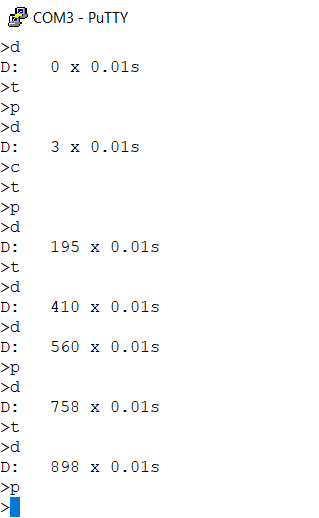
\includegraphics{capture}
	\caption{Terminal screen capture}
	\label{fig:capture1}
\end{figure}

Figure \ref{fig:capture1} shows the output of the terminal after each prompt command was used in various steps. The screen capture mainly shows the timer increasing its counter as time goes on. Meanwhile, the user can print the value of the counter or pause it as needed.

\section*{Conclusion}
This laboratory exercise was useful in exploring hardware driven timing funcitonality. It was important to keep in mind performance of subroutines so that the timing functionality could be as accurate as possible. This exercise was successful as the desired functionality was implemented as demostrated in Figure \ref{fig:capture1}.

\label{LastPage}
\end{document}
